%==================== Ordforklaring ====================

\section{Ordforklaring} \label{sec:ordforklaring}

\subsubsection{System}
Det totale system indeholder bil, software på PC og kommunikation mellem Bil og PC. På bilen er der flere underblokke såsom PSoC 4 Pioneer kit, Raspberry Pi 2 og PCB'er udviklet til dette projekt.

\subsubsection{HID - Human Interface Device}
Et interface som en bruger anvender til at interagere med en computer fx. tastetur og mus. I dette projekt anvendes desuden en Xbox-360 controller, med følgende funktionalitet der er beskrevet i afsnit \ref{sec:swdesign_xboxcontroller} \nameref{sec:swdesign_xboxcontroller} på side \pageref{sec:swdesign_xboxcontroller}.

\begin{figure}[h]
	\centering
	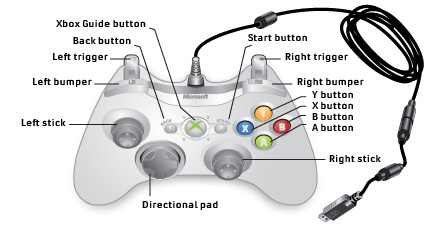
\includegraphics[width=\textwidth*4/5]{../fig/billeder/Wired-controller-callouts.jpg}
	\caption{Xbox-360 controller}
	\label{fig:xboxcontroller}
\end{figure}

\textbf{Forkortelser på knapper}
\begin{packed_item}
	\item RT - Right trigger
	\item LT - Left trigger 
	\item LS - Left stick
	\item RS - Right stick
\end{packed_item}
%TODO Er der brugt andre forkortelser?

\subsubsection{Hovedvindue}
Hovedvinduet i software på PC indeholder videostream, status på bilen samt muligheder for at konfigurere og kalibrere systemet.

\subsubsection{Bil}
Med bil menes den hardware der fysisk er placeret på bilen, dette være sig bla. bilens controllerenhed, her et Raspberry Pi 2 board, afstandsensorer, tachometer samt accelerometer.

\subsubsection{Pi - Raspberry Pi 2 B}
En Raspberry Pi er en single board computer i kreditkortstørrelse. Den anvendes i dette system som en controller til at styre bilen med.

\subsubsection{Wi-Fi netværk}
Trådløst netværk af standarden ''IEEE 802.11'', som Bil og PC kommunikerer over. Dette netværk sættes op lokalt til brug udelukkende for kommunikationen imellem Bil og PC. Der kan for eksempel anvendes et Wi-Fi hotspot fra en smartphone.

\subsubsection{AKS - Anti-kollitionssystem}
Et system på bilen bestående af fire afstandssensorer, samt signalbehandling- og reguleringssoftware som er i stand til at forhindre en kollision ved at overtage styring fra Bruger i tilfælde af forestående kollision. Der differentieres mellem "Undvig forhindring" og "Tænd/Sluk AKS".

\begin{itemize}
	\item Tænd/Sluk bruges i forbindelse med at koble AKS til eller fra, således at bilen ikke vil undgå en kollision hvis AKS er slukket, men vil undgå en kollision hvis AKS er tændt. 
	\item Undvig forhindring bruges i forbindelse med en forestående kollision. Her overtager AKS styring af bilen indtil forhindringen er undveget. 
\end{itemize}

\subsubsection{Afstandssensorer}
Afstandssensorerne er de 4 ultralydssensorer der er påmonteret bilen. Disse kan herefter benævnes som følgende:
\begin{packed_item}
	\item FL - Front left
	\item FR - Front right
	\item RL - Rear left
	\item RR - Rear right
\end{packed_item}

\subsubsection{UC - Use Case}
En use case er en standard for et brugsmønster til at afdække funktionalitet for et system.

\subsubsection{G - Tyngdeaccekeration}
G er tyngdeaccelerationen og har enheden $m/s^2$. $1G=9.81 m/s2$

\clearpage